\subsection{Room \& tenant relationship}
\label{sec:application:building_the_model:room_tenant_relationship}

In the thirteenth step, a relationship between two objects is introduced. This is the first step in which a relation is introduced between existing objects. For this relation, a object of $.\type{Room}$ may reference a single $.\type{Tenant}$ object. \cref{subsec:library_of_transformations:type_level_transformations:nullable_class_fields} is used to introduce the field on the type level, while on the instance level, \cref{subsec:library_of_transformations:instance_level_transformations:nullable_class_field_values} is used to introduce the values.

The $classtype$ of the new field is $.\type{Room}$, as the field will be defined for rooms. The $name$ of the new field is $\type{tenant}$ and the $fieldtype$ is $.\type{Tenant}$. The set of objects that will receive a value is defined as $valobjects = \{TRRoom1, TRRoom2, BHPRoomA, BHPRoomC\}$, while the set of objects that will not receive a value is defined as $nilobjects = \{BHPRoomB\}$. The union of these sets is equal to all the room objects, as expected. The function for $obids$ returns the existing identifier of each of these objects. The $values$ function is defined as follows:
\begin{align*}
    values = \{&(TRRoom1, Tenant1), (TRRoom2, Tenant2), (BHPRoomA, Tenant3), \\&(BHPRoomC, Tenant4)\}
\end{align*}

For the objects referenced by the objects in $valobjects$, the function $obids$ returns their existing identifier. The following model is obtained:

\LTXtable{\textwidth}{tex/06_application/02_building_the_model/tables/13_room_tenant_relationship.tex}

\begin{figure}[p]
    \centering
    \begin{subfigure}{0.98\textwidth}
        \centering
        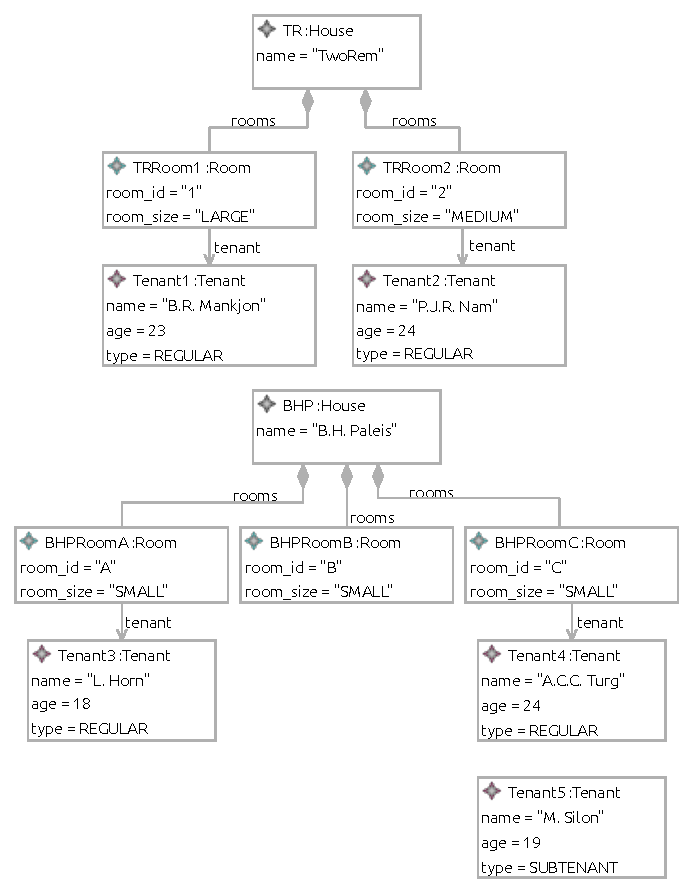
\includegraphics{images/06_application/instance_model/step13.pdf}
        \caption{Instance Model $Im_{13}$}
        \label{fig:application:building_the_model:room_tenant_relationship:ecore:instance_model}
    \end{subfigure}
    \\
    \begin{subfigure}{0.98\textwidth}
        \centering
        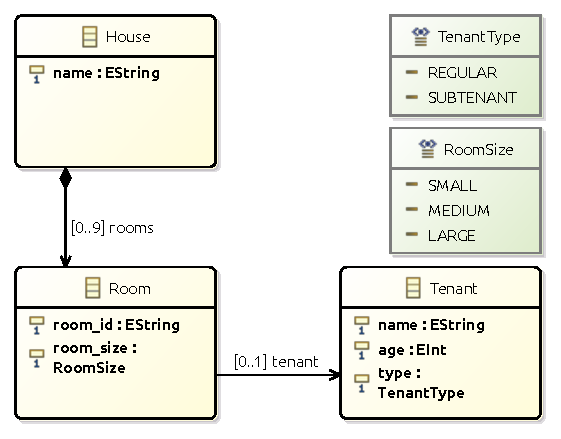
\includegraphics{images/06_application/type_model/step13.pdf}
        \caption{Type Model $Tm_{13}$}
        \label{fig:application:building_the_model:room_tenant_relationship:ecore:type_model}
    \end{subfigure}
    \caption{The Ecore model after step 13}
    \label{fig:application:building_the_model:room_tenant_relationship:ecore}
\end{figure}

\begin{figure}[p]
    \centering
    \begin{subfigure}{0.98\textwidth}
        \centering
        % To use this figure in your LaTeX document
% import the package groove/resources/groove2tikz.sty
%
\begin{tikzpicture}[scale=\tikzscale,name prefix=step13-]
\node[basic_node] (n0) at (2.825, -6.365) {\ml{\uline{\textit{BHP}} : \textbf{House}\\name = "B.H. Paleis"}};
\node[basic_node] (n1) at (2.655, -0.335) {\ml{\uline{\textit{TR}} : \textbf{House}\\name = "TwoRem"}};
\node[basic_node] (n2) at (2.575, -3.405) {\ml{\uline{\textit{RegularType}} : \textbf{TenantType\$REGULAR}}};
\node[basic_node] (n3) at (5.180, -1.965) {\ml{\uline{\textit{SubtenantType}} : \textbf{TenantType\$SUBTENANT}}};
\node[basic_node] (n4) at (2.845, -4.230) {\ml{\uline{\textit{SmallSize}} : \textbf{RoomSize}\\\textit{SMALL}}};
\node[basic_node] (n5) at (4.405, -0.570) {\ml{\uline{\textit{MediumSize}} : \textbf{RoomSize}\\\textit{MEDIUM}}};
\node[basic_node] (n6) at (0.990, -0.550) {\ml{\uline{\textit{LargeSize}} : \textbf{RoomSize}\\\textit{LARGE}}};
\node[basic_node] (n7) at (1.815, -1.465) {\ml{\uline{\textit{TRRoom1}} : \textbf{Room}\\room\_id = "1"}};
\node[basic_node] (n8) at (3.405, -1.475) {\ml{\uline{\textit{TRRoom2}} : \textbf{Room}\\room\_id = "2"}};
\node[basic_node] (n9) at (1.805, -2.475) {\ml{\uline{\textit{Tenant1}} : \textbf{Tenant}\\age = 23\\name = "B.R. Mankjon"}};
\node[basic_node] (n10) at (3.405, -2.475) {\ml{\uline{\textit{Tenant2}} : \textbf{Tenant}\\age = 24\\name = "P.J.R. Nam"}};
\node[basic_node] (n11) at (0.945, -4.285) {\ml{\uline{\textit{Tenant3}} : \textbf{Tenant}\\age = 18\\name = "L. Horn"}};
\node[basic_node] (n12) at (4.735, -4.225) {\ml{\uline{\textit{Tenant4}} : \textbf{Tenant}\\age = 24\\name = "A.C.C. Turg"}};
\node[basic_node] (n13) at (4.825, -3.275) {\ml{\uline{\textit{Tenant5}} : \textbf{Tenant}\\age = 19\\name = "M. Silon"}};
\node[basic_node] (n14) at (0.910, -5.225) {\ml{\uline{\textit{BHPRoomA}} : \textbf{Room}\\room\_id = "A"}};
\node[basic_node] (n15) at (2.870, -5.215) {\ml{\uline{\textit{BHPRoomB}} : \textbf{Room}\\room\_id = "B"}};
\node[basic_node] (n16) at (4.810, -5.225) {\ml{\uline{\textit{BHPRoomC}} : \textbf{Room}\\room\_id = "C"}};

\path[basic_edge] (n1)  -- node[lab] {\ml{rooms}} (n7) ;
\path[basic_edge](n16.north -| 4.735, -4.225) -- node[lab] {\ml{tenant}} (n12) ;
\path[basic_edge] (n0)  --  (n14) 
node[lab] at (1.960, -5.820) {\ml{rooms}};
\path[basic_edge](n15.north -| 2.845, -4.230) -- node[lab] {\ml{room\_size}} (n4) ;
\path[basic_edge] (n9)  -- node[lab] {\ml{type}}(n2.north -| 1.805, -2.475);
\path[basic_edge] (n8)  -- node[lab] {\ml{room\_size}} (n5) ;
\path[basic_edge] (n10)  -- node[lab] {\ml{type}}(n2.north -| 3.405, -2.475);
\path[basic_edge](n14.north -| 0.945, -4.285) -- node[lab] {\ml{tenant}} (n11) ;
\path[basic_edge](n0.north -| 2.870, -5.215) -- node[lab] {\ml{rooms}} (n15) ;
\path[basic_edge](n8.south -| 3.405, -2.475) -- node[lab] {\ml{tenant}} (n10) ;
\path[basic_edge] (n1)  -- node[lab] {\ml{rooms}} (n8) ;
\path[basic_edge] (n12)  -- node[lab] {\ml{type}} (n2) ;
\path[basic_edge] (n11)  -- node[lab] {\ml{type}} (n2) ;
\path[basic_edge] (n14)  -- node[lab] {\ml{room\_size}} (n4) ;
\path[basic_edge] (n0)  -- node[lab] {\ml{rooms}} (n16) ;
\path[basic_edge] (n7)  -- node[lab] {\ml{room\_size}} (n6) ;
\path[basic_edge](n13.north -| 5.180, -1.965) -- node[lab] {\ml{type}} (n3) ;
\path[basic_edge](n7.south -| 1.805, -2.475) -- node[lab] {\ml{tenant}} (n9) ;
\path[basic_edge] (n16)  -- node[lab] {\ml{room\_size}} (n4) ;
\end{tikzpicture}

        \caption{Instance Graph $IG_{13}$}
        \label{fig:application:building_the_model:room_tenant_relationship:groove:instance_graph}
    \end{subfigure}
    \\
    \begin{subfigure}{0.98\textwidth}
        \centering
        % To use this figure in your LaTeX document
% import the package groove/resources/groove2tikz.sty
%
\begin{tikzpicture}[scale=\tikzscale,name prefix=step13-]
\node[basic_node] (n0) at (2.825, -6.365) {\ml{\uline{\textit{BHP}} : \textbf{House}\\name = "B.H. Paleis"}};
\node[basic_node] (n1) at (2.655, -0.335) {\ml{\uline{\textit{TR}} : \textbf{House}\\name = "TwoRem"}};
\node[basic_node] (n2) at (2.575, -3.405) {\ml{\uline{\textit{RegularType}} : \textbf{TenantType\$REGULAR}}};
\node[basic_node] (n3) at (5.180, -1.965) {\ml{\uline{\textit{SubtenantType}} : \textbf{TenantType\$SUBTENANT}}};
\node[basic_node] (n4) at (2.845, -4.230) {\ml{\uline{\textit{SmallSize}} : \textbf{RoomSize}\\\textit{SMALL}}};
\node[basic_node] (n5) at (4.405, -0.570) {\ml{\uline{\textit{MediumSize}} : \textbf{RoomSize}\\\textit{MEDIUM}}};
\node[basic_node] (n6) at (0.990, -0.550) {\ml{\uline{\textit{LargeSize}} : \textbf{RoomSize}\\\textit{LARGE}}};
\node[basic_node] (n7) at (1.815, -1.465) {\ml{\uline{\textit{TRRoom1}} : \textbf{Room}\\room\_id = "1"}};
\node[basic_node] (n8) at (3.405, -1.475) {\ml{\uline{\textit{TRRoom2}} : \textbf{Room}\\room\_id = "2"}};
\node[basic_node] (n9) at (1.805, -2.475) {\ml{\uline{\textit{Tenant1}} : \textbf{Tenant}\\age = 23\\name = "B.R. Mankjon"}};
\node[basic_node] (n10) at (3.405, -2.475) {\ml{\uline{\textit{Tenant2}} : \textbf{Tenant}\\age = 24\\name = "P.J.R. Nam"}};
\node[basic_node] (n11) at (0.945, -4.285) {\ml{\uline{\textit{Tenant3}} : \textbf{Tenant}\\age = 18\\name = "L. Horn"}};
\node[basic_node] (n12) at (4.735, -4.225) {\ml{\uline{\textit{Tenant4}} : \textbf{Tenant}\\age = 24\\name = "A.C.C. Turg"}};
\node[basic_node] (n13) at (4.825, -3.275) {\ml{\uline{\textit{Tenant5}} : \textbf{Tenant}\\age = 19\\name = "M. Silon"}};
\node[basic_node] (n14) at (0.910, -5.225) {\ml{\uline{\textit{BHPRoomA}} : \textbf{Room}\\room\_id = "A"}};
\node[basic_node] (n15) at (2.870, -5.215) {\ml{\uline{\textit{BHPRoomB}} : \textbf{Room}\\room\_id = "B"}};
\node[basic_node] (n16) at (4.810, -5.225) {\ml{\uline{\textit{BHPRoomC}} : \textbf{Room}\\room\_id = "C"}};

\path[basic_edge] (n1)  -- node[lab] {\ml{rooms}} (n7) ;
\path[basic_edge](n16.north -| 4.735, -4.225) -- node[lab] {\ml{tenant}} (n12) ;
\path[basic_edge] (n0)  --  (n14) 
node[lab] at (1.960, -5.820) {\ml{rooms}};
\path[basic_edge](n15.north -| 2.845, -4.230) -- node[lab] {\ml{room\_size}} (n4) ;
\path[basic_edge] (n9)  -- node[lab] {\ml{type}}(n2.north -| 1.805, -2.475);
\path[basic_edge] (n8)  -- node[lab] {\ml{room\_size}} (n5) ;
\path[basic_edge] (n10)  -- node[lab] {\ml{type}}(n2.north -| 3.405, -2.475);
\path[basic_edge](n14.north -| 0.945, -4.285) -- node[lab] {\ml{tenant}} (n11) ;
\path[basic_edge](n0.north -| 2.870, -5.215) -- node[lab] {\ml{rooms}} (n15) ;
\path[basic_edge](n8.south -| 3.405, -2.475) -- node[lab] {\ml{tenant}} (n10) ;
\path[basic_edge] (n1)  -- node[lab] {\ml{rooms}} (n8) ;
\path[basic_edge] (n12)  -- node[lab] {\ml{type}} (n2) ;
\path[basic_edge] (n11)  -- node[lab] {\ml{type}} (n2) ;
\path[basic_edge] (n14)  -- node[lab] {\ml{room\_size}} (n4) ;
\path[basic_edge] (n0)  -- node[lab] {\ml{rooms}} (n16) ;
\path[basic_edge] (n7)  -- node[lab] {\ml{room\_size}} (n6) ;
\path[basic_edge](n13.north -| 5.180, -1.965) -- node[lab] {\ml{type}} (n3) ;
\path[basic_edge](n7.south -| 1.805, -2.475) -- node[lab] {\ml{tenant}} (n9) ;
\path[basic_edge] (n16)  -- node[lab] {\ml{room\_size}} (n4) ;
\end{tikzpicture}

        \caption{Type Graph $TG_{13}$}
        \label{fig:application:building_the_model:room_tenant_relationship:groove:type_graph}
    \end{subfigure}
    \caption{The GROOVE graphs after step 13}
    \label{fig:application:building_the_model:room_tenant_relationship:groove}
\end{figure}

A visual representation of $Tm_{13}$ and $Im_{13}$ can be found in \cref{fig:application:building_the_model:room_tenant_relationship:ecore}. Similarly, a visual representation of $TG_{13}$ and $IG_{13}$ can be found in \cref{fig:application:building_the_model:room_tenant_relationship:groove}. Please note that because of the definitions of $f_{13}(Im_{13})$ and $f'_{13}(IG_{13})$, we have that $f_{13}(Im_{13}) = IG_{13}$ and $f'_{13}(IG_{13}) = Im_{13}$. Furthermore, $f_{13}(Im_{13})$ and $f'_{13}(IG_{13})$ are valid mapping functions themselves, such that they can be combined with another mapping function in the next step.

The visualisation shows the references between the rooms and the tenants. This transformation shows how existing objects can be referenced by a new field, while also showing that values can be null. For example, $BHPRoomB$ has no tenant, which can be seen by the absence of a $tenant$ relation in the visualisation.

\afterpage{\FloatBarrier}